% Generated by Sphinx.
\def\sphinxdocclass{report}
\documentclass[letterpaper,10pt,english]{sphinxmanual}
\usepackage[utf8]{inputenc}
\DeclareUnicodeCharacter{00A0}{\nobreakspace}
\usepackage[T1]{fontenc}
\usepackage{babel}
\usepackage{times}
\usepackage[Bjarne]{fncychap}
\usepackage{longtable}
\usepackage{sphinx}
\usepackage{multirow}


\title{takahe Documentation}
\date{February 20, 2013}
\release{0.33}
\author{Florian Boudin}
\newcommand{\sphinxlogo}{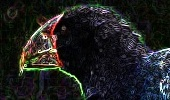
\includegraphics{takahe.jpg}\par}
\renewcommand{\releasename}{Release}
\makeindex

\makeatletter
\def\PYG@reset{\let\PYG@it=\relax \let\PYG@bf=\relax%
    \let\PYG@ul=\relax \let\PYG@tc=\relax%
    \let\PYG@bc=\relax \let\PYG@ff=\relax}
\def\PYG@tok#1{\csname PYG@tok@#1\endcsname}
\def\PYG@toks#1+{\ifx\relax#1\empty\else%
    \PYG@tok{#1}\expandafter\PYG@toks\fi}
\def\PYG@do#1{\PYG@bc{\PYG@tc{\PYG@ul{%
    \PYG@it{\PYG@bf{\PYG@ff{#1}}}}}}}
\def\PYG#1#2{\PYG@reset\PYG@toks#1+\relax+\PYG@do{#2}}

\expandafter\def\csname PYG@tok@gd\endcsname{\def\PYG@tc##1{\textcolor[rgb]{0.63,0.00,0.00}{##1}}}
\expandafter\def\csname PYG@tok@gu\endcsname{\let\PYG@bf=\textbf\def\PYG@tc##1{\textcolor[rgb]{0.50,0.00,0.50}{##1}}}
\expandafter\def\csname PYG@tok@gt\endcsname{\def\PYG@tc##1{\textcolor[rgb]{0.00,0.27,0.87}{##1}}}
\expandafter\def\csname PYG@tok@gs\endcsname{\let\PYG@bf=\textbf}
\expandafter\def\csname PYG@tok@gr\endcsname{\def\PYG@tc##1{\textcolor[rgb]{1.00,0.00,0.00}{##1}}}
\expandafter\def\csname PYG@tok@cm\endcsname{\let\PYG@it=\textit\def\PYG@tc##1{\textcolor[rgb]{0.25,0.50,0.56}{##1}}}
\expandafter\def\csname PYG@tok@vg\endcsname{\def\PYG@tc##1{\textcolor[rgb]{0.73,0.38,0.84}{##1}}}
\expandafter\def\csname PYG@tok@m\endcsname{\def\PYG@tc##1{\textcolor[rgb]{0.13,0.50,0.31}{##1}}}
\expandafter\def\csname PYG@tok@mh\endcsname{\def\PYG@tc##1{\textcolor[rgb]{0.13,0.50,0.31}{##1}}}
\expandafter\def\csname PYG@tok@cs\endcsname{\def\PYG@tc##1{\textcolor[rgb]{0.25,0.50,0.56}{##1}}\def\PYG@bc##1{\setlength{\fboxsep}{0pt}\colorbox[rgb]{1.00,0.94,0.94}{\strut ##1}}}
\expandafter\def\csname PYG@tok@ge\endcsname{\let\PYG@it=\textit}
\expandafter\def\csname PYG@tok@vc\endcsname{\def\PYG@tc##1{\textcolor[rgb]{0.73,0.38,0.84}{##1}}}
\expandafter\def\csname PYG@tok@il\endcsname{\def\PYG@tc##1{\textcolor[rgb]{0.13,0.50,0.31}{##1}}}
\expandafter\def\csname PYG@tok@go\endcsname{\def\PYG@tc##1{\textcolor[rgb]{0.20,0.20,0.20}{##1}}}
\expandafter\def\csname PYG@tok@cp\endcsname{\def\PYG@tc##1{\textcolor[rgb]{0.00,0.44,0.13}{##1}}}
\expandafter\def\csname PYG@tok@gi\endcsname{\def\PYG@tc##1{\textcolor[rgb]{0.00,0.63,0.00}{##1}}}
\expandafter\def\csname PYG@tok@gh\endcsname{\let\PYG@bf=\textbf\def\PYG@tc##1{\textcolor[rgb]{0.00,0.00,0.50}{##1}}}
\expandafter\def\csname PYG@tok@ni\endcsname{\let\PYG@bf=\textbf\def\PYG@tc##1{\textcolor[rgb]{0.84,0.33,0.22}{##1}}}
\expandafter\def\csname PYG@tok@nl\endcsname{\let\PYG@bf=\textbf\def\PYG@tc##1{\textcolor[rgb]{0.00,0.13,0.44}{##1}}}
\expandafter\def\csname PYG@tok@nn\endcsname{\let\PYG@bf=\textbf\def\PYG@tc##1{\textcolor[rgb]{0.05,0.52,0.71}{##1}}}
\expandafter\def\csname PYG@tok@no\endcsname{\def\PYG@tc##1{\textcolor[rgb]{0.38,0.68,0.84}{##1}}}
\expandafter\def\csname PYG@tok@na\endcsname{\def\PYG@tc##1{\textcolor[rgb]{0.25,0.44,0.63}{##1}}}
\expandafter\def\csname PYG@tok@nb\endcsname{\def\PYG@tc##1{\textcolor[rgb]{0.00,0.44,0.13}{##1}}}
\expandafter\def\csname PYG@tok@nc\endcsname{\let\PYG@bf=\textbf\def\PYG@tc##1{\textcolor[rgb]{0.05,0.52,0.71}{##1}}}
\expandafter\def\csname PYG@tok@nd\endcsname{\let\PYG@bf=\textbf\def\PYG@tc##1{\textcolor[rgb]{0.33,0.33,0.33}{##1}}}
\expandafter\def\csname PYG@tok@ne\endcsname{\def\PYG@tc##1{\textcolor[rgb]{0.00,0.44,0.13}{##1}}}
\expandafter\def\csname PYG@tok@nf\endcsname{\def\PYG@tc##1{\textcolor[rgb]{0.02,0.16,0.49}{##1}}}
\expandafter\def\csname PYG@tok@si\endcsname{\let\PYG@it=\textit\def\PYG@tc##1{\textcolor[rgb]{0.44,0.63,0.82}{##1}}}
\expandafter\def\csname PYG@tok@s2\endcsname{\def\PYG@tc##1{\textcolor[rgb]{0.25,0.44,0.63}{##1}}}
\expandafter\def\csname PYG@tok@vi\endcsname{\def\PYG@tc##1{\textcolor[rgb]{0.73,0.38,0.84}{##1}}}
\expandafter\def\csname PYG@tok@nt\endcsname{\let\PYG@bf=\textbf\def\PYG@tc##1{\textcolor[rgb]{0.02,0.16,0.45}{##1}}}
\expandafter\def\csname PYG@tok@nv\endcsname{\def\PYG@tc##1{\textcolor[rgb]{0.73,0.38,0.84}{##1}}}
\expandafter\def\csname PYG@tok@s1\endcsname{\def\PYG@tc##1{\textcolor[rgb]{0.25,0.44,0.63}{##1}}}
\expandafter\def\csname PYG@tok@gp\endcsname{\let\PYG@bf=\textbf\def\PYG@tc##1{\textcolor[rgb]{0.78,0.36,0.04}{##1}}}
\expandafter\def\csname PYG@tok@sh\endcsname{\def\PYG@tc##1{\textcolor[rgb]{0.25,0.44,0.63}{##1}}}
\expandafter\def\csname PYG@tok@ow\endcsname{\let\PYG@bf=\textbf\def\PYG@tc##1{\textcolor[rgb]{0.00,0.44,0.13}{##1}}}
\expandafter\def\csname PYG@tok@sx\endcsname{\def\PYG@tc##1{\textcolor[rgb]{0.78,0.36,0.04}{##1}}}
\expandafter\def\csname PYG@tok@bp\endcsname{\def\PYG@tc##1{\textcolor[rgb]{0.00,0.44,0.13}{##1}}}
\expandafter\def\csname PYG@tok@c1\endcsname{\let\PYG@it=\textit\def\PYG@tc##1{\textcolor[rgb]{0.25,0.50,0.56}{##1}}}
\expandafter\def\csname PYG@tok@kc\endcsname{\let\PYG@bf=\textbf\def\PYG@tc##1{\textcolor[rgb]{0.00,0.44,0.13}{##1}}}
\expandafter\def\csname PYG@tok@c\endcsname{\let\PYG@it=\textit\def\PYG@tc##1{\textcolor[rgb]{0.25,0.50,0.56}{##1}}}
\expandafter\def\csname PYG@tok@mf\endcsname{\def\PYG@tc##1{\textcolor[rgb]{0.13,0.50,0.31}{##1}}}
\expandafter\def\csname PYG@tok@err\endcsname{\def\PYG@bc##1{\setlength{\fboxsep}{0pt}\fcolorbox[rgb]{1.00,0.00,0.00}{1,1,1}{\strut ##1}}}
\expandafter\def\csname PYG@tok@kd\endcsname{\let\PYG@bf=\textbf\def\PYG@tc##1{\textcolor[rgb]{0.00,0.44,0.13}{##1}}}
\expandafter\def\csname PYG@tok@ss\endcsname{\def\PYG@tc##1{\textcolor[rgb]{0.32,0.47,0.09}{##1}}}
\expandafter\def\csname PYG@tok@sr\endcsname{\def\PYG@tc##1{\textcolor[rgb]{0.14,0.33,0.53}{##1}}}
\expandafter\def\csname PYG@tok@mo\endcsname{\def\PYG@tc##1{\textcolor[rgb]{0.13,0.50,0.31}{##1}}}
\expandafter\def\csname PYG@tok@mi\endcsname{\def\PYG@tc##1{\textcolor[rgb]{0.13,0.50,0.31}{##1}}}
\expandafter\def\csname PYG@tok@kn\endcsname{\let\PYG@bf=\textbf\def\PYG@tc##1{\textcolor[rgb]{0.00,0.44,0.13}{##1}}}
\expandafter\def\csname PYG@tok@o\endcsname{\def\PYG@tc##1{\textcolor[rgb]{0.40,0.40,0.40}{##1}}}
\expandafter\def\csname PYG@tok@kr\endcsname{\let\PYG@bf=\textbf\def\PYG@tc##1{\textcolor[rgb]{0.00,0.44,0.13}{##1}}}
\expandafter\def\csname PYG@tok@s\endcsname{\def\PYG@tc##1{\textcolor[rgb]{0.25,0.44,0.63}{##1}}}
\expandafter\def\csname PYG@tok@kp\endcsname{\def\PYG@tc##1{\textcolor[rgb]{0.00,0.44,0.13}{##1}}}
\expandafter\def\csname PYG@tok@w\endcsname{\def\PYG@tc##1{\textcolor[rgb]{0.73,0.73,0.73}{##1}}}
\expandafter\def\csname PYG@tok@kt\endcsname{\def\PYG@tc##1{\textcolor[rgb]{0.56,0.13,0.00}{##1}}}
\expandafter\def\csname PYG@tok@sc\endcsname{\def\PYG@tc##1{\textcolor[rgb]{0.25,0.44,0.63}{##1}}}
\expandafter\def\csname PYG@tok@sb\endcsname{\def\PYG@tc##1{\textcolor[rgb]{0.25,0.44,0.63}{##1}}}
\expandafter\def\csname PYG@tok@k\endcsname{\let\PYG@bf=\textbf\def\PYG@tc##1{\textcolor[rgb]{0.00,0.44,0.13}{##1}}}
\expandafter\def\csname PYG@tok@se\endcsname{\let\PYG@bf=\textbf\def\PYG@tc##1{\textcolor[rgb]{0.25,0.44,0.63}{##1}}}
\expandafter\def\csname PYG@tok@sd\endcsname{\let\PYG@it=\textit\def\PYG@tc##1{\textcolor[rgb]{0.25,0.44,0.63}{##1}}}

\def\PYGZbs{\char`\\}
\def\PYGZus{\char`\_}
\def\PYGZob{\char`\{}
\def\PYGZcb{\char`\}}
\def\PYGZca{\char`\^}
\def\PYGZam{\char`\&}
\def\PYGZlt{\char`\<}
\def\PYGZgt{\char`\>}
\def\PYGZsh{\char`\#}
\def\PYGZpc{\char`\%}
\def\PYGZdl{\char`\$}
\def\PYGZhy{\char`\-}
\def\PYGZsq{\char`\'}
\def\PYGZdq{\char`\"}
\def\PYGZti{\char`\~}
% for compatibility with earlier versions
\def\PYGZat{@}
\def\PYGZlb{[}
\def\PYGZrb{]}
\makeatother

\begin{document}

\maketitle
\tableofcontents
\phantomsection\label{index::doc}

\phantomsection\label{index:module-takahe}\index{takahe (module)}\begin{quote}\begin{description}
\item[{Name}] \leavevmode
takahe

\item[{Authors}] \leavevmode
Florian Boudin (\href{mailto:florian.boudin@univ-nantes.fr}{florian.boudin@univ-nantes.fr})

\item[{Version}] \leavevmode
0.33

\item[{Date}] \leavevmode
Feb. 2013

\item[{Description}] \leavevmode
takahe is a multi-sentence compression module. Given a set of redundant 
sentences, a word-graph is constructed by iteratively adding sentences to 
it. The best compression is obtained by finding the shortest path in the
word graph. The original algorithm was published and described in:
\begin{quote}

Katja Filippova, Multi-Sentence Compression: Finding Shortest Paths
in Word Graphs, \emph{Proceedings of the 23rd International Conference on 
Computational Linguistics (Coling 2010)}, pages 322-330, 2010.
\end{quote}

\item[{History}] \leavevmode\begin{itemize}
\item {} 
0.33 (Feb. 2013), bug fixes and better code documentation

\item {} 
0.32 (Jun. 2012), Punctuation marks are now considered within the graph, 
compressions are then punctuated

\item {} 
0.31 (Nov. 2011), modified context function (uses the left and right 
contexts), improved docstring documentation, bug fixes

\item {} 
0.3 (Oct. 2011), improved K-shortest paths algorithm including verb/size 
constraints and ordered lists for performance

\item {} 
0.2 (Dec. 2010), removed dependencies from nltk (i.e. POS-tagging, 
tokenization and stopwords removal)

\item {} 
0.1 (Nov. 2010), first version

\end{itemize}

\item[{Dependencies}] \leavevmode\begin{itemize}
\item {} 
\emph{networkx} for the graph construction (v1.2+)

\end{itemize}

\item[{Usage}] \leavevmode
A typical usage of this module is:

\begin{Verbatim}[commandchars=\\\{\}]
\PYG{k+kn}{import} \PYG{n+nn}{takahe}

\PYG{c}{\PYGZsh{} A list of tokenized and POS\PYGZhy{}tagged sentences}
\PYG{n}{sentences} \PYG{o}{=} \PYG{p}{[}\PYG{l+s}{\PYGZsq{}}\PYG{l+s}{Hillary/NNP Clinton/NNP wanted/VBD to/stop visit/VB ...}\PYG{l+s}{\PYGZsq{}}\PYG{p}{]}

\PYG{c}{\PYGZsh{} Create a word graph from the set of sentences with parameters :}
\PYG{c}{\PYGZsh{} \PYGZhy{} minimal number of words in the compression : 6}
\PYG{c}{\PYGZsh{} \PYGZhy{} language of the input sentences : en (english)}
\PYG{c}{\PYGZsh{} \PYGZhy{} POS tag for punctuation marks : PUNCT}
\PYG{n}{compresser} \PYG{o}{=} \PYG{n}{takahe}\PYG{o}{.}\PYG{n}{word\PYGZus{}graph}\PYG{p}{(}\PYG{n}{sentences}\PYG{p}{,} \PYG{l+m+mi}{6}\PYG{p}{,} \PYG{l+s}{\PYGZsq{}}\PYG{l+s}{en}\PYG{l+s}{\PYGZsq{}}\PYG{p}{,} \PYG{l+s}{\PYGZdq{}}\PYG{l+s}{PUNCT}\PYG{l+s}{\PYGZdq{}}\PYG{p}{)}

\PYG{c}{\PYGZsh{} Get the 50 best paths}
\PYG{n}{candidates} \PYG{o}{=} \PYG{n}{compresser}\PYG{o}{.}\PYG{n}{get\PYGZus{}compression}\PYG{p}{(}\PYG{l+m+mi}{5}\PYG{p}{)}

\PYG{c}{\PYGZsh{} Rerank compressions by path length}
\PYG{k}{for} \PYG{n}{cummulative\PYGZus{}score}\PYG{p}{,} \PYG{n}{path} \PYG{o+ow}{in} \PYG{n}{candidates}\PYG{p}{:}

    \PYG{c}{\PYGZsh{} Normalize path score by path length}
    \PYG{n}{normalized\PYGZus{}score} \PYG{o}{=} \PYG{n}{cummulative\PYGZus{}score} \PYG{o}{/} \PYG{n+nb}{len}\PYG{p}{(}\PYG{n}{path}\PYG{p}{)}

    \PYG{c}{\PYGZsh{} Print normalized score and compression}
    \PYG{k}{print} \PYG{n+nb}{round}\PYG{p}{(}\PYG{n}{normalized\PYGZus{}score}\PYG{p}{,} \PYG{l+m+mi}{3}\PYG{p}{)}\PYG{p}{,} \PYG{l+s}{\PYGZsq{}}\PYG{l+s}{ }\PYG{l+s}{\PYGZsq{}}\PYG{o}{.}\PYG{n}{join}\PYG{p}{(}\PYG{p}{[}\PYG{n}{u}\PYG{p}{[}\PYG{l+m+mi}{0}\PYG{p}{]} \PYG{k}{for} \PYG{n}{u} \PYG{o+ow}{in} \PYG{n}{path}\PYG{p}{]}\PYG{p}{)}

\PYG{c}{\PYGZsh{} Write the word graph in the dot format}
\PYG{n}{compresser}\PYG{o}{.}\PYG{n}{write\PYGZus{}dot}\PYG{p}{(}\PYG{l+s}{\PYGZsq{}}\PYG{l+s}{test.dot}\PYG{l+s}{\PYGZsq{}}\PYG{p}{)}
\end{Verbatim}

\item[{Misc}] \leavevmode
The Takahe is a flightless bird indigenous to New Zealand. It was thought to
be extinct after the last four known specimens were taken in 1898. However, 
after a carefully planned search effort the bird was rediscovered by on 
November 20, 1948. (Wikipedia, \href{http://en.wikipedia.org/wiki/takahe}{http://en.wikipedia.org/wiki/takahe})

\end{description}\end{quote}


\chapter{word\_graph class}
\label{index:word-graph-class}\label{index:takahe-documentation}\index{word\_graph (class in takahe)}

\begin{fulllineitems}
\phantomsection\label{index:takahe.word_graph}\pysiglinewithargsret{\strong{class }\code{takahe.}\bfcode{word\_graph}}{\emph{sentence\_list}, \emph{nb\_words=8}, \emph{lang='en'}, \emph{punct\_tag='PUNCT'}}{}
The word\_graph class constructs a word graph from the set of sentences given
as input. The set of sentences is a list of strings, sentences are tokenized
and words are POS-tagged (e.g. \code{"Saturn/NNP is/VBZ the/DT sixth/JJ 
planet/NN from/IN the/DT Sun/NNP in/IN the/DT Solar/NNP System/NNP"}). 
Three optional parameters can be specified. The first parameter is the 
minimal number of words for the best compression (default value is 8). The 
second parameter is the language and is used for selecting the correct 
stopwords list (default is ``en'' for english, stopword lists are localized in 
/resources/ directory). The third parameter is the punctuation mark tag 
used during graph construction (default is PUNCT).
\index{ambiguous\_nodes() (takahe.word\_graph method)}

\begin{fulllineitems}
\phantomsection\label{index:takahe.word_graph.ambiguous_nodes}\pysiglinewithargsret{\bfcode{ambiguous\_nodes}}{\emph{node}}{}
Takes a node in parameter and returns the number of possible candidate 
(ambiguous) nodes in the graph.

\end{fulllineitems}

\index{build\_graph() (takahe.word\_graph method)}

\begin{fulllineitems}
\phantomsection\label{index:takahe.word_graph.build_graph}\pysiglinewithargsret{\bfcode{build\_graph}}{}{}
Constructs a directed word graph from the list of input sentences. Each
sentence is iteratively added to the directed graph according to the 
following algorithm:
\begin{itemize}
\item {} 
Word mapping/creation is done in four steps:
\begin{enumerate}
\item {} 
non-stopwords for which no candidate exists in the graph or for 
which an unambiguous mapping is possible or which occur more than
once in the sentence

\item {} 
non-stopwords for which there are either several possible
candidates in the graph

\item {} 
stopwords

\item {} 
punctuation marks

\end{enumerate}

\end{itemize}

For the last three groups of words where mapping is ambiguous we check 
the immediate context (the preceding and following words in the sentence 
and the neighboring nodes in the graph) and select the candidate which 
has larger overlap in the context, or the one with a greater frequency 
(i.e. the one which has more words mapped onto it). Stopwords are mapped 
only if there is some overlap in non-stopwords neighbors, otherwise a 
new node is created. Punctuation marks are mapped only if the preceding 
and following words in the sentence and the neighboring nodes are the
same.
\begin{itemize}
\item {} 
Edges are then computed and added between mapped words.

\end{itemize}

Each node in the graph is represented as a tuple (`word/POS', id) and 
possesses an info list containing (sentence\_id, position\_in\_sentence)
tuples.

\end{fulllineitems}

\index{compute\_statistics() (takahe.word\_graph method)}

\begin{fulllineitems}
\phantomsection\label{index:takahe.word_graph.compute_statistics}\pysiglinewithargsret{\bfcode{compute\_statistics}}{}{}
This function iterates over the cluster's sentences and computes the
following statistics about each word:
\begin{itemize}
\item {} 
term frequency (self.term\_freq)

\end{itemize}

\end{fulllineitems}

\index{get\_compression() (takahe.word\_graph method)}

\begin{fulllineitems}
\phantomsection\label{index:takahe.word_graph.get_compression}\pysiglinewithargsret{\bfcode{get\_compression}}{\emph{nb\_candidates=50}}{}
Searches all possible paths from \textbf{start} to \textbf{end} in the word graph,
removes paths containing no verb or shorter than \emph{n} words. Returns an
ordered list (smaller first) of nb (default value is 50) (cummulative 
score, path) tuples. The score is not normalized with the sentence 
length.

\end{fulllineitems}

\index{get\_directed\_context() (takahe.word\_graph method)}

\begin{fulllineitems}
\phantomsection\label{index:takahe.word_graph.get_directed_context}\pysiglinewithargsret{\bfcode{get\_directed\_context}}{\emph{node}, \emph{k}, \emph{dir='all'}, \emph{non\_pos=False}}{}
Returns the directed context of a given node, i.e. a list of word/POS of
the left or right neighboring nodes in the graph. The function takes 
four parameters :
\begin{itemize}
\item {} 
node is the word/POS tuple

\item {} 
k is the node identifier used when multiple nodes refer to the same 
word/POS (e.g. k=0 for (the/DET, 0), k=1 for (the/DET, 1), etc.)

\item {} 
dir is the parameter that controls the directed context calculation, 
it can be set to left, right or all (default)

\item {} 
non\_pos is a boolean allowing to remove stopwords from the context 
(default is false)

\end{itemize}

\end{fulllineitems}

\index{get\_edge\_weight() (takahe.word\_graph method)}

\begin{fulllineitems}
\phantomsection\label{index:takahe.word_graph.get_edge_weight}\pysiglinewithargsret{\bfcode{get\_edge\_weight}}{\emph{node1}, \emph{node2}}{}
Compute the weight of an edge \emph{e} between nodes \emph{node1} and \emph{node2}. It 
is computed as e\_ij = (A / B) / C with:
\begin{itemize}
\item {} 
A = freq(i) + freq(j),

\item {} 
B = Sum (s in S) 1 / diff(s, i, j)

\item {} 
C = freq(i) * freq(j)

\end{itemize}

A node is a tuple of (`word/POS', unique\_id).

\end{fulllineitems}

\index{graph (takahe.word\_graph attribute)}

\begin{fulllineitems}
\phantomsection\label{index:takahe.word_graph.graph}\pysigline{\bfcode{graph}\strong{ = None}}
The directed graph used for fusion.

\end{fulllineitems}

\index{k\_shortest\_paths() (takahe.word\_graph method)}

\begin{fulllineitems}
\phantomsection\label{index:takahe.word_graph.k_shortest_paths}\pysiglinewithargsret{\bfcode{k\_shortest\_paths}}{\emph{start}, \emph{end}, \emph{k=10}}{}
Simple implementation of a k-shortest paths algorithms. Takes three
parameters: the starting node, the ending node and the number of 
shortest paths desired. Returns a list of k tuples (path, weight).

\end{fulllineitems}

\index{length (takahe.word\_graph attribute)}

\begin{fulllineitems}
\phantomsection\label{index:takahe.word_graph.length}\pysigline{\bfcode{length}\strong{ = None}}
The number of sentences given for fusion.

\end{fulllineitems}

\index{load\_stopwords() (takahe.word\_graph method)}

\begin{fulllineitems}
\phantomsection\label{index:takahe.word_graph.load_stopwords}\pysiglinewithargsret{\bfcode{load\_stopwords}}{\emph{path}}{}
This function loads a stopword list from the \emph{path} file and returns a 
set of words. Lines begining by `\#' are ignored.

\end{fulllineitems}

\index{max\_index() (takahe.word\_graph method)}

\begin{fulllineitems}
\phantomsection\label{index:takahe.word_graph.max_index}\pysiglinewithargsret{\bfcode{max\_index}}{\emph{l}}{}
Returns the index of the maximum value of a given list.

\end{fulllineitems}

\index{nb\_words (takahe.word\_graph attribute)}

\begin{fulllineitems}
\phantomsection\label{index:takahe.word_graph.nb_words}\pysigline{\bfcode{nb\_words}\strong{ = None}}
The minimal number of words in the compression.

\end{fulllineitems}

\index{pre\_process\_sentences() (takahe.word\_graph method)}

\begin{fulllineitems}
\phantomsection\label{index:takahe.word_graph.pre_process_sentences}\pysiglinewithargsret{\bfcode{pre\_process\_sentences}}{}{}
Pre-process the list of sentences given as input. Split sentences using 
whitespaces and convert each sentence to a list of (word, POS) tuples.

\end{fulllineitems}

\index{punct\_tag (takahe.word\_graph attribute)}

\begin{fulllineitems}
\phantomsection\label{index:takahe.word_graph.punct_tag}\pysigline{\bfcode{punct\_tag}\strong{ = None}}
The stopword tag used in the graph.

\end{fulllineitems}

\index{resources (takahe.word\_graph attribute)}

\begin{fulllineitems}
\phantomsection\label{index:takahe.word_graph.resources}\pysigline{\bfcode{resources}\strong{ = None}}
The path of the resources folder.

\end{fulllineitems}

\index{sentence (takahe.word\_graph attribute)}

\begin{fulllineitems}
\phantomsection\label{index:takahe.word_graph.sentence}\pysigline{\bfcode{sentence}\strong{ = None}}
A list of sentences provided by the user.

\end{fulllineitems}

\index{sep (takahe.word\_graph attribute)}

\begin{fulllineitems}
\phantomsection\label{index:takahe.word_graph.sep}\pysigline{\bfcode{sep}\strong{ = None}}
The separator used between a word and its POS in the graph.

\end{fulllineitems}

\index{start (takahe.word\_graph attribute)}

\begin{fulllineitems}
\phantomsection\label{index:takahe.word_graph.start}\pysigline{\bfcode{start}\strong{ = None}}
The start token in the graph.

\end{fulllineitems}

\index{stop (takahe.word\_graph attribute)}

\begin{fulllineitems}
\phantomsection\label{index:takahe.word_graph.stop}\pysigline{\bfcode{stop}\strong{ = None}}
The end token in the graph.

\end{fulllineitems}

\index{stopword\_path (takahe.word\_graph attribute)}

\begin{fulllineitems}
\phantomsection\label{index:takahe.word_graph.stopword_path}\pysigline{\bfcode{stopword\_path}\strong{ = None}}
The path of the stopword list, e.g. stopwords.{[}lang{]}.dat.

\end{fulllineitems}

\index{stopwords (takahe.word\_graph attribute)}

\begin{fulllineitems}
\phantomsection\label{index:takahe.word_graph.stopwords}\pysigline{\bfcode{stopwords}\strong{ = None}}
The set of stopwords loaded from stopwords.{[}lang{]}.dat.

\end{fulllineitems}

\index{term\_freq (takahe.word\_graph attribute)}

\begin{fulllineitems}
\phantomsection\label{index:takahe.word_graph.term_freq}\pysigline{\bfcode{term\_freq}\strong{ = None}}
The frequency of a given term.

\end{fulllineitems}

\index{verbs (takahe.word\_graph attribute)}

\begin{fulllineitems}
\phantomsection\label{index:takahe.word_graph.verbs}\pysigline{\bfcode{verbs}\strong{ = None}}
The list of verb POS tags required in the compression. At least \emph{one}
verb must occur in the candidate compressions.

\end{fulllineitems}

\index{write\_dot() (takahe.word\_graph method)}

\begin{fulllineitems}
\phantomsection\label{index:takahe.word_graph.write_dot}\pysiglinewithargsret{\bfcode{write\_dot}}{\emph{dotfile}}{}
Outputs the word graph in dot format in the specified file.

\end{fulllineitems}


\end{fulllineitems}



\chapter{Indices and tables}
\label{index:indices-and-tables}\begin{itemize}
\item {} 
\emph{genindex}

\item {} 
\emph{modindex}

\item {} 
\emph{search}

\end{itemize}


\renewcommand{\indexname}{Python Module Index}
\begin{theindex}
\def\bigletter#1{{\Large\sffamily#1}\nopagebreak\vspace{1mm}}
\bigletter{t}
\item {\texttt{takahe}}, \pageref{index:module-takahe}
\end{theindex}

\renewcommand{\indexname}{Index}
\printindex
\end{document}
